\section{Asymptotic results}\label{asymptotic-sec}

In this section we use the effective estimates from Theorem \ref{eff} to obtain asymptotic information about the function $H_t$, which improves (and makes more effective) the results of Ki, Kim, and Lee \cite{kkl}, by establishing Theorem \ref{Zero}.

We begin with an asymptotic

\begin{proposition}\label{asymp}  Let $0 < t \leq 1/2$, $x \geq 200$, and $-10 \leq y \leq 10$.
\begin{itemize}
\item[(i)]  If $x \geq \exp(\frac{C}{t})$ for a sufficiently large absolute constant $C$, then
$$ H_t(x+iy) = (1 + O(x^{-ct})) M_t\left(\frac{1+y-ix}{2}\right) + (1 + O(x^{-ct})) M_t\left(\frac{1-y+ix}{2} \right) $$
for an absolute constant $c>0$, where $M_t$ is defined in \eqref{Mt-def}.  
\item[(ii)]  If instead we have $3 \leq y \leq 4$ and $x \geq C$ for a sufficiently large absolute constant $C$, then
$$ H_t(x+iy) = (1 + O_{\leq}(0.7)) M_t\left(\frac{1+y-ix}{2}\right).$$
\item[(iii)]  If $x = x_0 + O(1)$ for some $x_0 \geq 200$, then
$$ H_t(x+iy) = O( x_0^{O(1)} |M_t(\frac{1+y-ix}{2})| ) = O( x_0^{O(1)} |M_t(\frac{ix_0}{2})| ).$$
\end{itemize}
\end{proposition}

\begin{proof}  We begin with (i).  Since $H_t = H_t^*$ and $M_t = M_t^*$, we may assume without loss of generality that $y \geq 0$.
Using \eqref{lambda-def}, \eqref{bo-def} we may write the desired estimate as
$$ \frac{H_t(x+iy)}{B_0(x+iy)} = 1 + O(x^{-ct}) + \gamma.$$
We apply Theorem \ref{eff}.  (Strictly speaking, the estimates there required $y \leq 1$ rather than $y \leq 10$; however, as remarked at the beginning of Section \ref{initial-sec}, all the estimates in that section would continue to hold under this weaker hypothesis if one adjusted all the numerical constants appropriately.)  This gives
\begin{equation}\label{exp}
\frac{H_t(x+iy)}{B_0(x+iy)} = \sum_{n=1}^N \frac{b_n^t}{n^{s_*}} + \gamma \sum_{n=1}^N n^y \frac{b_n^t}{n^{\overline{s_*} + \kappa}} + O_{\leq}\left( e_A + e_B + e_{C,0} \right)
\end{equation}
where
\begin{align*}
\gamma &= O( x^{-y/2} ) \\
\kappa &= O(x^{-1}) \\
\mathrm{Re}(s_*) &\geq \frac{1+y}{2} + \frac{t}{2} \log \frac{x}{4\pi}  - O(x^{-2}) \\
e_A &= O\left( x^{-y/2} \sum_{n=1}^N b_n^t n^{-\frac{1-y}{2} - \frac{t}{2} \log \frac{x}{4\pi} - O(x^{-1})} \frac{\log^2 x}{x} \right) \\ 
e_B &= O\left( \sum_{n=1}^N b_n^t n^{-\frac{1+y}{2} - \frac{t}{2} \log \frac{x}{4\pi} + O(x^{-1})} \frac{\log^2 x}{x} \right) \\ 
e_{C,0} &= O\left( x^{-\frac{1+y}{4}} \right)
\end{align*}
Since $N = O(x^{1/2})$, we have $x^{-y/2} n^{y} = O(1)$ and $n^{O(x^{-1})} = O(1)$ for all $1 \leq n \leq N$.  We conclude that
$$\frac{H_t(x+iy)}{B_0(x+iy)} = 1 + \gamma + O\left( \frac{\log^2 x}{x} + \sum_{n=2}^N \frac{b_n^t}{n^{\frac{1+y}{2} + \frac{t}{2} \log \frac{x}{4\pi}}} + x^{-\frac{1+y}{4}} \right) $$
so it will suffice (for $c$ small enough) to show that
$$ \sum_{n=2}^N \frac{b_n^t}{n^{\frac{1+y}{2} + \frac{t}{2} \log \frac{x}{4\pi}}} = O( x^{-ct} ).$$
By \eqref{bn-def} we can write the left-hand side as
$$ \sum_{n=2}^N \frac{1}{n^{\frac{1+y}{2} + \frac{t}{2} \log \frac{x}{4\pi \sqrt{n}}}} = O( x^{-ct} ).$$
For $2 \leq n \leq N$, we have
$$ \frac{1+y}{2} + \frac{t}{2} \log \frac{x}{4\pi \sqrt{n}} \geq c t \log x $$
for some absolute constant $c>0$.  By the integral test, the left-hand side is then bounded by
$$ \frac{1}{2^{c t \log x}} + \int_2^\infty \frac{1}{u^{c t \log x}}\ du$$
which, for $x \geq \exp(C/t)$ and $C$ large, is bounded by $O(2^{-ct\log x})$.  The claim then follows after adjusting $c$ appropriately.

Now we prove (ii).  As before we have the expansion \eqref{exp}.  We have
\begin{align*}
\gamma \sum_{n=1}^N n^y \frac{b_n^t}{n^{\overline{s_*} + \kappa}} &= O\left( x^{-y/2} \sum_{n=1}^N \frac{b_n^t}{n^{-\frac{1-y}{2} + \frac{t}{2} \log \frac{x}{4\pi}}} \right) \\
&= O\left( x^{-y/2} \sum_{n=1}^N n^{\frac{y-1}{2}} \right) \\
&= O(x^{-\frac{y-1}{4}});
\end{align*}
similar arguments give $e_A = O( \frac{\log^2 x}{x^{\frac{y-1}{4}}} )$, while
\begin{align*}
e_B &= O\left( \frac{\log^2 x}{x} \sum_{n=1}^N b_n^t n^{-\frac{1+y}{2}-\frac{t}{2} \log \frac{x}{4\pi}} \right) \\
&= O\left( \frac{\log^2 x}{x} \sum_{n=1}^N n^{-2} \right) \\
&= O\left( \frac{\log^2 x}{x} \right).
\end{align*}
We conclude that
\begin{align*}
\frac{H_t(x+yi)}{B_0(x+yi)} &= \sum_{n=1}^N \frac{b_n^t}{n^{s_*}} + O( x^{-\frac{y-1}{4}} ) \\
&= 1 + O_{\leq}\left( \sum_{n=2}^N n^{-\frac{1+y}{2} - \frac{t}{2} \log \frac{x}{4\pi} - O(x^{-1})} \right) + O( x^{\frac{y-1}{4}} ) \\
&= 1 + O_{\leq}\left( \sum_{n=2}^N n^{-2} \right) + O( x^{-1/2}) \\
&= 1 + O_{\leq}\left( \frac{\pi^2}{6} - 1 \right) + O( x^{-1/2} ) \\
&= 1 + O_{\leq}( 0.7 )
\end{align*}
as claimed, if $x \geq C$ for $C$ large enough.

Finally we prove (iii).  Again our starting point is \eqref{exp}.  The right-hand side can be bounded crudely by $O( x^{O(1)}) = O(x_0^{O(1)})$, hence
$$ H_t(x+iy) = O( x_0^{O(1)} |M_t( \frac{1+y+ix}{2} )| ).$$
However, from \eqref{Mt-def}, \eqref{M-def}, \eqref{alpha-form} it is not hard to see that the log-derivative of $M_t(s)$ is of size $O( \log x_0 )$ in the region $s = \frac{ix_0}{2} + O(1)$.  Thus
$$ |M_t( \frac{1+y+ix}{2} )| = O( x_0^{O(1)} |M_t( \frac{ix_0}{2} )| ),$$
giving the claim.
\end{proof}

To understand the behavior of $M_t(x+iy)$ we make the following simple observations:

\begin{lemma}\label{mtform}  Let $0 < t \leq 1/2$, let $x_* > 0$ be sufficiently large, and let $x+iy = x_* + O(1)$.  Then
$$ M_t(\frac{1+y+ix}{2}) = M_t(\frac{1+ix_*}{2}) \exp\left( (i(x-x_*)+y) \left(\frac{1}{4} \log \frac{x_*}{4\pi} + \frac{\pi i}{8}\right) + O\left( \frac{\log x_*}{x_*}\right) \right).$$
Also, there is a continuous branch of $\mathrm{arg} M_t\left(\frac{1+ix_*}{2}\right)$ for all large real $x_*$ such that
$$ \mathrm{arg} M_t\left(\frac{1+ix_*}{2}\right) = \frac{t \pi}{16} \log \frac{x_*}{4\pi} + \frac{7\pi}{8} 
+ \frac{x_*}{4} \log \frac{x_*}{4\pi} - \frac{x_*}{4} + O( \frac{\log x_*}{x_*} ).$$
\end{lemma}

\begin{proof}
By \eqref{Mt-def}, \eqref{alpha-def}, the log-derivative of $M_t$ is given by
\begin{equation}\label{mt-deriv}
 \frac{M'_t}{M_t} = \alpha + \frac{t}{2} \alpha \alpha'.
\end{equation}
For $s = \frac{ix_*}{2} + O(1)$, we have from \eqref{alpha-form} that
\begin{equation}\label{alpha-ex}
\alpha(s) = \frac{1}{2} \log \frac{x_*}{4\pi} + \frac{\pi i}{4} + O\left( \frac{1}{x_*}\right) 
\end{equation}
and from this and \eqref{alpha-deriv-bound} we conclude that
$$
 \frac{M'_t(s)}{M_t(s)} = \frac{1}{2} \log \frac{x_*}{4\pi} + \frac{\pi i}{4} + O\left( \frac{\log x_*}{x_*}\right) $$
whenever $s = \frac{ix_*}{2} + O(1)$.  The first claim then follows by applying the fundamental theorem of calculus to a branch of $\log M_t$.

For the second claim, we calculate
\begin{align*}
\mathrm{arg} M_t\left(\frac{1+ix_*}{2}\right) &= \frac{t}{4} \mathrm{Im} \alpha\left(\frac{1+ix_*}{2}\right)^2 + \pi - \frac{x_*}{4} \log \pi + \mathrm{Im}\left( \frac{-1+ix_*}{4} \log \frac{1+ix_*}{4} - \frac{1+ix_*}{4}\right) \\
&= \frac{t}{4} \left(\frac{\pi}{4} \log \frac{x_*}{4\pi} + O(\frac{\log x_*}{x_*})\right) + \pi - \frac{x_*}{4} \log \pi 
+ \mathrm{Im}\left( \frac{-1+ix_*}{4} \left(\log \frac{x_*}{4} + \frac{i\pi}{2} - \frac{i}{x_*} + O\left(\frac{1}{x_*^2}\right) \right) \right) - \frac{x_*}{4} \\
&= \frac{t \pi}{16} \log \frac{x_*}{4\pi} + \pi + \frac{x_*}{4} \log \pi 
+ \frac{x_*}{4} \log \frac{x_*}{4} - \frac{\pi}{8} + O\left( \frac{\log x_*}{x_*} \right) \\
&= \frac{t \pi}{16} \log \frac{x_*}{4\pi} + \frac{7\pi}{8} 
+ \frac{x_*}{4} \log \frac{x_*}{4\pi} - \frac{x_*}{4} + O\left( \frac{\log x_*}{x_*} \right) 
\end{align*}
as desired.
\end{proof}

Now we can prove Theorem \ref{Zero}.  We begin with (ii).  Let $n \geq \exp( \frac{C}{t})$, and suppose that $x+iy = x_n + O(1)$.  
By Proposition \ref{asymp}(i) and Lemma \ref{mtform} we have
\begin{equation}\label{htap}
\begin{split}
 H_t(x+iy) &= \overline{M_t\left(\frac{1+ix_n}{2}\right)} \exp\left( (-i(x-x_n)+y) \left(\frac{1}{4} \log \frac{x_n}{4\pi} - \frac{\pi i}{8}\right) + O( x_n^{-ct} )\right)\\
&\quad  + M_t\left(\frac{1+ix_n}{2}\right) \exp\left( (i(x-x_n)-y) \left(\frac{1}{4} \log \frac{x_n}{4\pi} + \frac{\pi i}{8}\right) + O( x_n^{-ct} )\right).
\end{split}
\end{equation}
From Lemma \ref{mtform} and \eqref{lip} one has
$$ \mathrm{arg} M_t\left(\frac{1+ix_n}{2}\right)  = -\frac{\pi}{2} + O\left( \frac{\log x_n}{x_n} \right)\hbox{ mod } \pi $$
and hence 
\begin{equation}\label{ma}
\overline{M_t\left(\frac{1+ix_n}{2}\right)} = - \exp\left( O( \frac{\log x_n}{x_n} ) \right) M_t\left(\frac{1+ix_n}{2}\right).
\end{equation}
If we now make the further assumption $y = O\left( \frac{1}{\log x_n}\right)$, we can thus simplify the above approximation as
\begin{equation}\label{ht-eff}
\begin{split}
 H_t(x+iy) &= - M_t\left(\frac{1+ix_n}{2}\right) e^{-\pi (x-x_n)/8} \exp\left( (-i(x-x_n)+y) \frac{1}{4} \log \frac{x_n}{4\pi} + O( |y| \log x_n + x_n^{-ct} ) \right)\\
&\quad + M_t\left(\frac{1+ix_n}{2}\right) e^{-\pi (x-x_n)/8} \exp\left( (i(x-x_n)-y) \frac{1}{4} \log \frac{x_n}{4\pi} + O( |y| \log x_n + x_n^{-ct} ) \right)\\
&= 2 i M_t\left(\frac{1+ix_n}{2}\right) e^{-\pi (x-x_n)/8} \left( \sin\left(\frac{x+iy-x_n}{4} \log \frac{x_n}{4\pi}\right) + O( |y| \log x_n + x_n^{-ct} )\right ).
\end{split}
\end{equation}
In particular, if $x+iy$ traverses the circle $\{ x_n + \frac{c}{\log n} e^{i\theta}: 0 \leq \theta \leq 2\pi\}$ once anti-clockwise and $c$ is small enough, the quantity $H_t(x+iy)$ will wind exactly once around the origin, and hence by the argument principle there is precisely one zero of $H_t$ inside this circle.  As the zeroes of $H_t$ are symmetric around the real axis, this zero must be real.  This proves (ii).

Now we prove (i).
Suppose that $H_t(x+iy)=0$ and $x \geq \exp(\frac{C}{t})$.  We can assume $|y| \leq 1$ since it is known (e.g., from \cite[Theorem 13]{debr}) that there are no zeroes with $|y|>1$.  

Let $n$ be a natural number that minimises $|x-x_n|$, then $x = x_n+O\left(\frac{1}{\log x_n}\right)$ since the derivative of the left-hand side of \eqref{lip} in $x_n$ is comparable to $\log x_n$.  From \eqref{htap} we have
\begin{align*}
0 &= \overline{M_t\left(\frac{1+ix_n}{2}\right)} \exp\left( (-i(x-x_n)+y) \left(\frac{1}{4} \log \frac{x_n}{4\pi} - \frac{\pi i}{8}\right) + O( x_n^{-ct} )\right) \\
&\quad + M_t(\frac{1+ix_n}{2}) \exp\left( (i(x-x_n)-y) \left(\frac{1}{4} \log \frac{x_n}{4\pi} + \frac{\pi i}{8}\right) + O( x_n^{-ct} )\right).
\end{align*}
Thus both summands on the right-hand side have the same magnitude, which on taking logarithms and canceling like terms implies that
$$ y \frac{1}{4} \log \frac{x_n}{4\pi} + O( x_n^{-ct} ) = -y \frac{1}{4} \log \frac{x_n}{4\pi} + O( x_n^{-ct} )$$
and hence $y = O\left( \frac{x_n^{-ct}}{\log x_n} \right)$.  We can now apply \eqref{ht-eff} to conclude that
$$ \sin\left(\frac{x+iy-x_n}{4} \log \frac{x_n}{4\pi}\right) + O( x_n^{-ct} ) = 0$$
which (when combined with the hypothesis that $|x-x_n|$ is minimal) forces $x - x_n = O\left( \frac{x_n^{-ct}}{\log x_n} \right)$.  This gives the claim.

Next, we prove (iii).  In view of parts (i) and (ii), and adjusting $C$ if necessary, we may assume that $X$ takes the form $X = x_n+\frac{c}{\log x_n}$ for some $n \geq \exp( \frac{C}{t})$.  By the argument principle, $N_t(X)$ is equal to $\frac{-1}{2\pi}$ times the variation in the argument of $H_t$ on the boundary of the rectangle $\{ x+iy: 0 \leq x \leq X; -3 \leq y \leq 3 \}$ traversed clockwise, since there are no zeroes with imaginary part of magnitude greater than one.  By compactness, the variation on the left edge $\{ iy: -3 \leq y \leq 3 \}$ is $O(1)$, and similarly for any fixed portion $\{ x+3i: 0 \leq y \leq C \}$ of the upper edge.  From Proposition \ref{asymp} (and \eqref{htap}), we see that the variation of $H_t(x+iy) / M_t(\frac{1+y-ix}{2})$ on the remaining upper edge $\{ x+3i: C \leq x \leq X \}$ and on the top half $\{ X+iy: 0 \leq y \leq 3 \}$ of the right edge are both equal to $O(1)$.  Since $H_t = H_t^*$, the variation on the lower half of the rectangle is equal to that of the upper half. We thus conclude that
$$ N_t(X) = -\frac{1}{\pi} \mathrm{arg} M_t\left(\frac{1-iX}{2}\right)+ O(1)$$
where we use a continuous branch of the argument of $M_t\left(\frac{1-iX}{2}\right)$ that is bounded at $3i$.  The claim now follows from Lemma \ref{mtform}.

Finally, we prove (iv).  From \eqref{htdef} and the rapid decrease of $\Phi$ it is easy to verify that the entire function $H_t$ has order $1$, while from the positivity of $\Phi$ we see that $H_t$ has no zero at the origin.  Thus by the Hadamard factorization theorem we have
$$ H_t(z) = \exp(a+bz) \prod_n \left( 1 - \frac{z}{z_n} \right) \exp( \frac{z}{z_n} )$$
for some complex numbers $a,b$, where $z_n$ are the zeroes of $H_t$ counting multiplicity; using the functional equation $H_t(z) = H_t(-z)$ we can index the zeros as $z_n = (z_n)_{n \in \Z \backslash \{0\}}$ with $z_{-n} = -z_n$, and conclude that $b=0$, and
$$ H_t(z) = \exp(a) \prod_{n>0} \left( 1 - \frac{z^2}{z_n^2} \right).$$
Taking logarithmic derivatives, we conclude that
\begin{equation}\label{hata}
 \frac{H'_t(z)}{H_t(z)} = \sum_{n>0} \left(\frac{1}{z-z_n} + \frac{1}{z+z_n}\right).
\end{equation}
Setting $z = X+4i$, we see from Proposition \ref{asymp} and the generalized Cauchy integral formula that the logarithmic derivative of $H_t(x+iy)/M_t\left(\frac{1+y-ix}{2}\right)$ is equal to $O(1)$ at $X+4i$ for all sufficiently large $X$, and hence for all $X$ by symmetry and compactness.  On the other hand, from Stirling's formula (or the logarithmic growth of the digamma function) one easily verifies that the logarithmic derivative of $M_t\left(\frac{1+y-ix}{2}\right)$  is equal to $O( \log(2+X) )$ at $X+4i$.  Hence $\frac{H'_t(X+4i)}{H_t(X+4i)} = O(\log(2+X))$.  Taking imaginary parts, we conclude that
$$ \sum_{n>0} \frac{(4-y_n)}{(X-x_n)^2 + (4-y_n)^2} + \frac{(4-y_n)}{(X+x_n)^2 + (4+y_n)^2} = O(\log(2+X))$$
where we write $z_n = x_n + iy_n$; equivalently one has
$$ \sum_n \frac{(4-y_n)}{(X-x_n)^2 + (4-y_n)^2} = O(\log(2+X))$$
where the sum now ranges over all zeroes, including any at the origin. Since $|y_n| \leq 1$, every zero in $[X,X+1]$ makes a contribution of at least $\frac{1}{100}$ (say).  As the summands are all positive, the first part of claim (iv) follows.  To prove the second part, we may assume by compactness that $x \geq C$.  Repeating the proof of (iii), and reduce to showing that the variation of $\mathrm{arg} H_t$ on the short vertical interval $\{ X+iy: 0 \leq y \leq 3 \}$ is $O( \log X )$.  If we let $\theta$ be a phase such that $e^{i\theta} H_t(X+3i)$ is real and positive, we see that this variation is at most $\pi(m+1)$, where $m$ is the number of zeroes of $\mathrm{Re} e^{i\theta} H_t(X+yi)$ for $0 \leq y \leq 3$, since every increment of $\pi$ in $\mathrm{arg} e^{i\theta} H_t$ must be accompanied by at least one such zero.  As $H_t = H_t^*$, this is also the number of zeroes of $e^{i\theta} H_t(X+yi) + e^{-i\theta} H_t(2X - (X+yi))$.  On the other hand, from Proposition \ref{asymp}(ii), (iii) and Jensen's formula we see that the number of such zeroes is $O( \log X )$, and the claim follows.

\begin{remark}\label{time-complexity}  Theorem \ref{Zero} gives good control on $H_t(x+iy)$ whenever $x \geq \exp( C/t )$.  As a consequence (and assuming for sake of argument that the Riemann hypothesis holds), then for any $\Lambda_0 > 0$, the bound $\Lambda \leq \Lambda_0$ should be numerically verifiable in time $O( \exp( O(1/\Lambda_0) ))$, by applying the arguments of previous sections with $t$ and $y$ set equal to small multiples of $\Lambda_0$.  We leave the details to the interested reader.
\end{remark}

\begin{remark} Our discussion here will be informal.  In view of the results of \cite{csv}, it is expected that the zeroes $z_j(t)$ of $H_t(x+iy)$ should evolve according to the system of ordinary differential equations
$$ \partial_t z_k(t) = 2 \sum_{j \neq k}^{\prime} \frac{1}{z_k(t) - z_j(t)}$$
where the sum is evaluated in a suitable principal value sense, and one avoids those times where the zero $z_k(t)$ fails to be simple; see \cite[Lemma 2.4]{csv} for a verification of this in the regime $t > \Lambda$.  In view of the Riemann-von Mangoldt formula (as well as variants such Corollary \ref{Zero}, it is expected that the number of zeroes in any region of the form $\{ x+iy: x+iy = x_* + O(1) \}$ for large $x_*$ should be of the order of $\log x_*$.  As a consequence, we expect a typical zero $z_k(t)$ to move with speed $O( \log |z_k(t)| )$, although one may occasionally move much faster than this if two zeroes are exceptionally close together, or less than this if the zeroes are close to being evenly spaced.  As a consequence, if the Riemann hypothesis fails and there is a zero $x+iy$ of $H_0$ with $y$ comparable to $1$, it should take time comparable to $\frac{1}{\log x}$ for this zero to move towards the real axis, leading to the heuristic lower bound $\Lambda \gg \frac{1}{\log x}$.  Thus, in order to obtain an upper bound $\Lambda \leq \Lambda_0$, it will probably be necessary to verify that there are no zeroes $x+iy$ of $H_0$ with $y$ comparable to $1$ and $|x| \leq c \log \frac{1}{\Lambda}$ for some small absolute constant $c>0$.  This suggests that the time complexity bound in Remark \ref{time-complexity} is likely to be best possible (unless one is able to prove the Riemann hypothesis, of course).

In \cite[Lemma 2.1]{csv} it is also shown that the velocity of a given zero $z(t)$ is given by the formula
$$ \partial_t z(t) = \frac{H''_t(z(t))}{H'_t(z(t))}$$
assuming that the zero is simple.  By using the asymptotics in Proposition \ref{asymp} and Corollary \ref{Zero} together with the generalized Cauchy integral formula to then obtain asymptotics for $H'_t$ and $H''_t$, it is possible to show that for the zeroes $x(t)$ that are real and larger than $\exp(C/t)$, and move leftwards with velocity
$$ \partial_t x(t) = - \frac{\pi}{4} + O( x^{-ct} );$$
we leave the details to the interested reader.  

{\bf maybe supply some numerically computed graphics here?}
\begin{figure}[h!]
  \includegraphics[width=0.9\linewidth]{real_zeros_solid.png}
  \caption{Real zeros moving up leftwards and getting `solidified'.}
\end{figure}

\begin{figure}[h!]
  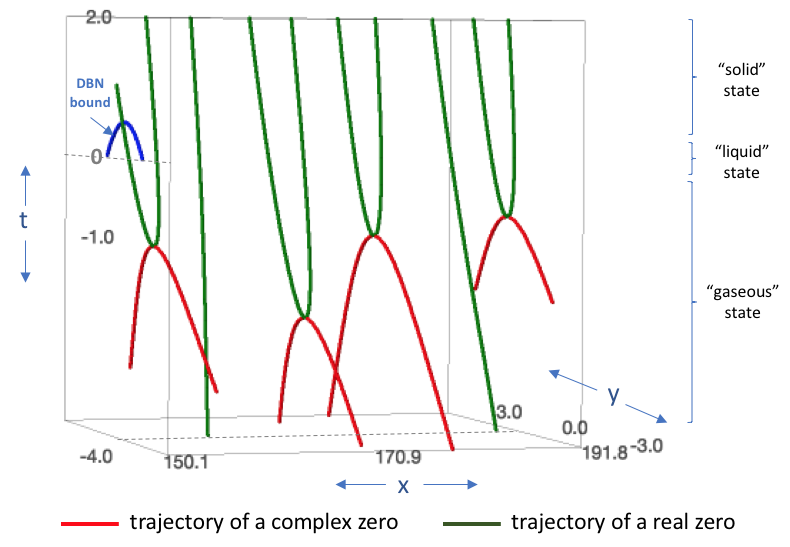
\includegraphics[width=0.9\linewidth]{Actual_trajectories_zeros.png}
  \caption{Actual trajectories of some real and complex zeros.}
\end{figure}

\end{remark}


